
\documentclass[preprint,12pt]{elsarticle}

%% Use the option review to obtain double line spacing
%\documentclass[preprint,review,12pt]{elsarticle}

%% Use the options 1p,twocolumn; 3p; 3p,twocolumn; 5p; or 5p,twocolumn
%% for a journal layout:
%% \documentclass[final,1p,times]{elsarticle}
%% \documentclass[final,1p,times,twocolumn]{elsarticle}
%% \documentclass[final,3p,times]{elsarticle}
%% \documentclass[final,3p,times,twocolumn]{elsarticle}
%% \documentclass[final,5p,times]{elsarticle}
%% \documentclass[final,5p,times,twocolumn]{elsarticle}

%% The graphicx package provides the includegraphics command.
\usepackage{graphicx}
%% The amssymb package provides various useful mathematical symbols
\usepackage{amssymb}
%% The amsthm package provides extended theorem environments
%% \usepackage{amsthm}

%% The lineno packages adds line numbers. Start line numbering with
%% \begin{linenumbers}, end it with \end{linenumbers}. Or switch it on
%% for the whole article with \linenumbers after \end{frontmatter}.
\usepackage{lineno}

%% natbib.sty is loaded by default. However, natbib options can be
%% provided with \biboptions{...} command. Following options are
%% valid:

%%   round  -  round parentheses are used (default)
%%   square -  square brackets are used   [option]
%%   curly  -  curly braces are used      {option}
%%   angle  -  angle brackets are used    <option>
%%   semicolon  -  multiple citations separated by semi-colon
%%   colon  - same as semicolon, an earlier confusion
%%   comma  -  separated by comma
%%   numbers-  selects numerical citations
%%   super  -  numerical citations as superscripts
%%   sort   -  sorts multiple citations according to order in ref. list
%%   sort&compress   -  like sort, but also compresses numerical citations
%%   compress - compresses without sorting
%%
%% \biboptions{comma,round}

% \biboptions{}

\journal{NeuroImage}

\begin{document}

\begin{frontmatter}
\title{An atlas-free method for group analysis of resting state fMRI using brainsync transform}

%% use the tnoteref command within \title for footnotes;
%% use the tnotetext command for the associated footnote;
%% use the fnref command within \author or \address for footnotes;
%% use the fntext command for the associated footnote;
%% use the corref command within \author for corresponding author footnotes;
%% use the cortext command for the associated footnote;
%% use the ead command for the email address,
%% and the form \ead[url] for the home page:
%%
%% \title{Title\tnoteref{label1}}
%% \tnotetext[label1]{}
%% \author{Name\corref{cor1}\fnref{label2}}
%% \ead{email address}
%% \ead[url]{home page}
%% \fntext[label2]{}
%% \cortext[cor1]{}
%% \address{Address\fnref{label3}}
%% \fntext[label3]{}



\author[usc]{Anand A. Joshi}
\author[usc]{Jian Li}
\author[usc]{Soyoung Choi}
\author[usc]{Haleh Akrami}
\author[usc]{Jonas Kaplan}
\author[usc]{Richard M. Leahy}

\address[usc]{University of Southern California, Los Angeles, USA}

\begin{abstract}
Resting fMRI (rfMRI) can provide insight into function of the human brain. However, due to spontaneous nature of the resting fMRI, the rfMRI scans cannot be compared across subjects.

We present a method for performing group studies of resting fMRI data based on brainsync transform. The proposed method uses ability to perform pairwise comparisons of fMRI scans using the brainsync transform and presents a statistical methodology for group analysis using pairwise comparisons of scans and clinical variables within the group. 
The proposed method is atlas-free and provides significantly improved sensitivity over atlas-based methods.
The methodology is applied to a group of ADHD and normal controls to identify brain regions associated with ADHD.

\end{abstract}

\begin{keyword}
fMRI \sep ADHD \sep Resting State \sep group differences
\end{keyword}

\end{frontmatter}
\linenumbers

\begin{enumerate}
    \item Perform Anatomical analysis also for the same population.
    
\end{enumerate}

\section{Introduction}
\label{sec:introduction}
The human brain exhibits intricate, complex and dynamic interactions among functional regions during resting offering insight into functional organization of the human brain. The fMRI signal acquired during resting (rfMRI) has been used extensively to measure functional connectivity between different brain regions \citep{horwitz_elusive_2003,lang_resting-state_2014,smith_network_2011, smitha_resting_2017,van_den_heuvel_exploring_2010}. It is also used for longitudinal studies of brain development and is as a diagnostic biomarker in cross-sectional studies for various neurological and psychological diseases and conditions \cite{redcay_intrinsic_2013}. 

Group studies of rfMRI involves averaging data across individuals in order to improve the signal-to-noise ratio (SNR) \cite{dubois_building_2016}. 
Since rfMRI data reflect spontaneous brain activity, it is not possible to directly compare resting state signals across subjects. Instead, comparisons make use of connectivity features \cite{iraji_connectivity_2016}, typically computed from pairwise correlations of the rfMRI time-series between a point of interest and other locations in the brain \cite{fan_human_2016}. For analysis of cerebral cortex, it is common to compute a feature vector at each location on a tessellated representation of the cortex as the correlation from that vertex to all other vertices. 

\section{Materials and Methods}
\label{sec:mat_methods}
\subsection{brainsync transform}

The recently developed Brainsync transform is an orthogonal transform
\cite{descoteaux_brainsync:_2017,joshi_are_2018} which can be used
for comparisons of fMRI scans across subjects that are collected during
resting state or task. In contrast with existing fMRI analysis methods,
this transform does not involve dimensionality reduction and also
preserves the rich dynamical information in fMRI scans. The method
is based on the observation that rfMRI data exhibit similar overall
connectivity patterns across subjects, as reflected in the pairwise
correlations between different brain regions (Figure \ref{fig:brainsync-transform-illustartion}).
As an input, the following illustration assumes preprocessed fMRI
data, sampled on the cortical surface or in the grayordinate coordinate
system developed by the Human Connectome Project team \cite{glasser_minimal_2013}.
The time series at each voxel was normalized to mean zero and unit
variance. Due to normalization, (zero mean, unit variance) the rfMRI
time series data can be represented as a set of labeled points on
the hypersphere. The similarity of resting connectivity patterns across
subjects (reflecting the existence of common networks: default mode,
visual, somatomotor, etc) results in clusters of points on the hypersphere,
separated from each other by a distance that reflects the correlation
between the corresponding time series. As a result, each subject's
data can be represented as a set of points on the hypersphere, differing
(approximately) across subjects by a rotation and or reflection of
the sphere. Alignment of time series across subjects can, therefore,
be approximately achieved by rotating their respective hyperspheres
so that they match. This process is illustrated in Figure \ref{fig:brainsync-transform-illustartion}
and is the basis for the BrainSync transform. The BrainSync mapping
between subjects requires the solution of a Procrustes least-squares
fit \cite{gower_procrustes_2004,ten_berge_orthogonal_1977} to compute
an orthogonal matrix of dimension equal to the number of images making
up the fMRI time-series. While the synchronization makes the time
courses of the two datasets similar, individual variation is retained
after the transformation as manifested in the differences in spatial
activation patterns between the reference and synchronized subject
data. This is to be expected and is an important feature of the proposed
transform: the BrainSync transform aligns the components of the spatiotemporal
data that are common (with respect to their representation in the
hypersphere) but also retains any individual differences. The BrainSync
transform is unique, invertible, efficient to compute, and preserves
the connectivity structure of the original data for all subjects.
Similar to image registration, where we spatially align the anatomical
brain images, synchronization of fMRI signals by the BrainSync transform,
across a population or within-subject across sessions, facilitates
longitudinal and cross-sectional studies of fMRI.

This transform was developed to be able to compare two resting state
scans, for within or across subjects. In its original form, it has
following limitations. 1. The scans that are being synchronized need
to have the same number of time points. The entire scans were `synchronized'
in order to compare them. 2. The temporal dynamics is not captured
within resting state, however across subject deviation from the average
dynamics can be captured.

In this work, we develop a weighted extension of the BrainSync transform
with a scaling factor, that facilitates study of temporal dynamics
within scan.

\begin{figure}
\begin{centering}
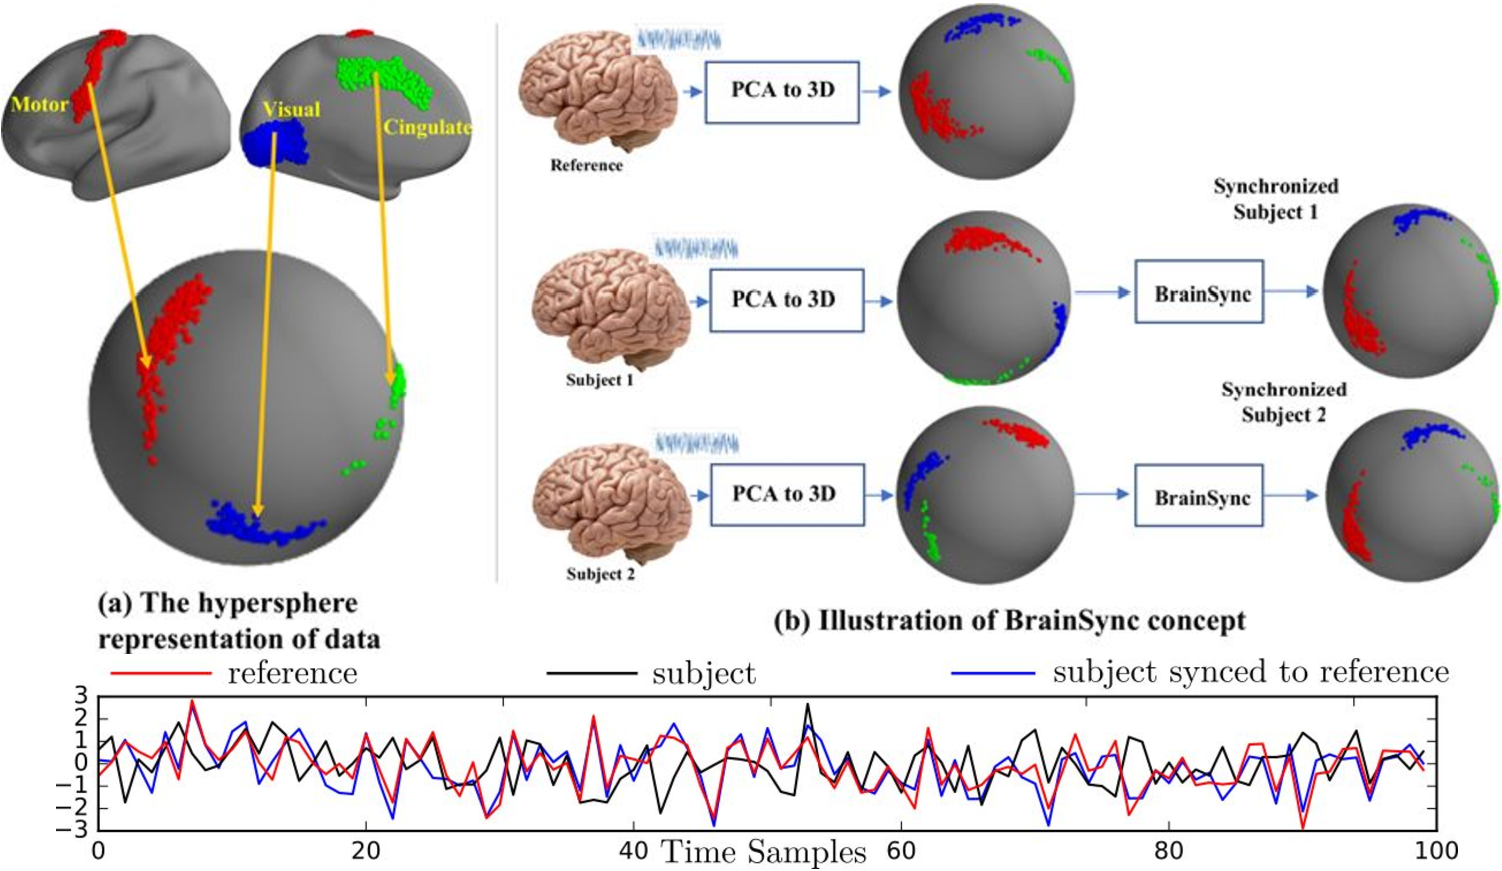
\includegraphics[width=1\textwidth]{figs/brainsync_concept} 
\par\end{centering}
\caption{Illustration of the BrainSync concept: (a) Data from motor (red),
cingulate (green) and visual (blue) areas was considered. Representation
of this data on a hypersphere is depicted. Dimensionality reduction
was performed using PCA. (b) Two datasets (subject and reference)
from these areas was used as input to PCA. Dimensionality of the data
was reduced to 3D and renormalized to generate the mapping to sphere.
Application of BrainSync to the subject results in a configuration
of data on the sphere very similar to that for the reference dataset.
The lower figure shows representative resting fMRI time-series for
two subjects for a single cortical location before and after synchronization.
Note the strong correlation of the blue and red time-series curves
from the two different subjects after synchronization. \label{fig:brainsync-transform-illustartion}}
\end{figure}

\subsection{Statistical analysis}
\subsubsection{Univariate statistic}
Synchronize all subjects to an atlas
Use distance to the atlas as a univariate feature
Correlate this statistic to clinical variable
Use Pearson correlation to compute p-value at each point on the cortex

We computed regression variable for subject i as 

Functional measure is norm of the distance of synced time series to average time series

Pearson correlation and p-value was computed at each vertex

\subsubsection{Multivariate statistic}

\subsubsection{Alternate Univariate Statistic}

In order to perform regression analysis
Consider 2000 random pairs of subjects
Synchronize one to the other 
Use norm square of the difference between their time series (fmri-diff)
Compute square of the difference between their clinical variables (var-diff)
Correlate fmri-diff to var-diff
Use Pearson correlation to compute p-value at each point in the grayordinates
Benjamini Hochberg FDR correction is done on the whole grayordinates


\section{Results}
\subsection{ADHD data and preprocessing}
ADHD200 dataset from fcon1000 was used and processed using BFP
50 normal controls were used to find a representative subject. Data from those  50 normal subjects was synced to the representative and averaged to form the ‘atlas’.
Another 150 subjects with Verbal IQ/ADHD index scores were used for comparison

\section{Discussion}

\section{Conclusion}
\label{S:2}


\bibliographystyle{model1-num-names}

\bibliography{sample.bib,zotero_ref.bib}


\end{document}

%%
%% End of file `elsarticle-template-1-num.tex'.